\section{Resultados}
\label{sec:resultados}

\subsection{Señales adquiridas y acondicionadas}
\label{sec:res-acondicionamiento}
% Responde: ítem 5
La figura~\ref{fig:acond_antes_despues} compara \SI{10}{\second} de cada registro antes y después del acondicionamiento. En reposo, el cambio principal es que la línea de base queda centrada en cero y plana; la forma de los complejos QRS y de las ondas T se conserva. En el registro post ejercicio el efecto es mucho mayor: la deriva de más de \SI{1}{\volt} desaparece y los complejos quedan alineados sobre una línea de base estable, salvo en el tramo saturado, que se interpoló y queda excluido del análisis. El espectro (figura~\ref{fig:acond_espectro_antes_despues}) muestra que la potencia por debajo de \SI{0.5}{\hertz} cae unos dos órdenes de magnitud, mientras que por encima de \SI{1}{\hertz} los espectros crudo y acondicionado coinciden.

\begin{figure}[htbp]
  \centering
  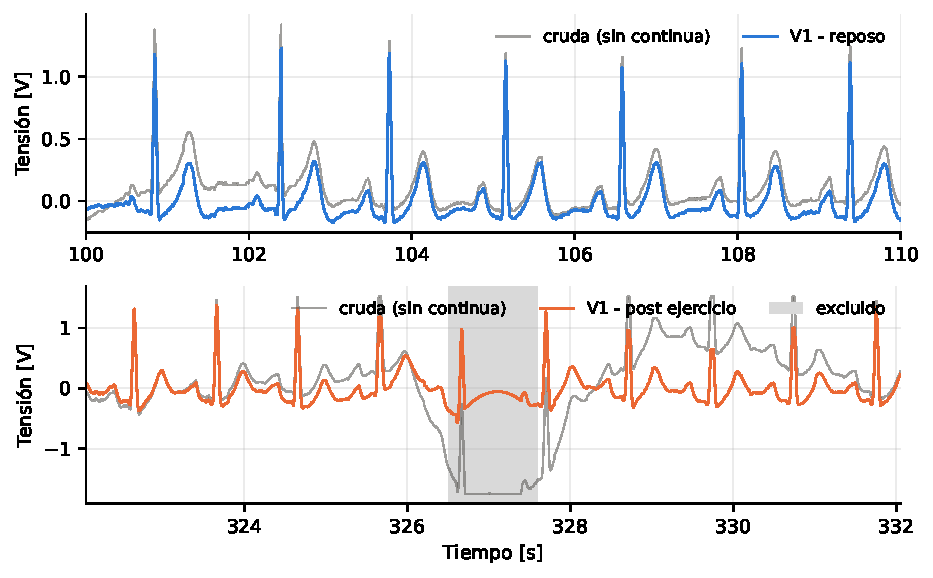
\includegraphics[width=\textwidth]{acond_antes_despues}
  \caption{Diez segundos de cada registro: señal cruda sin nivel de continua (gris) y acondicionada (color). En el registro post ejercicio, el sombreado marca un tramo saturado excluido del análisis.}
  \label{fig:acond_antes_despues}
\end{figure}

\begin{figure}[htbp]
  \centering
  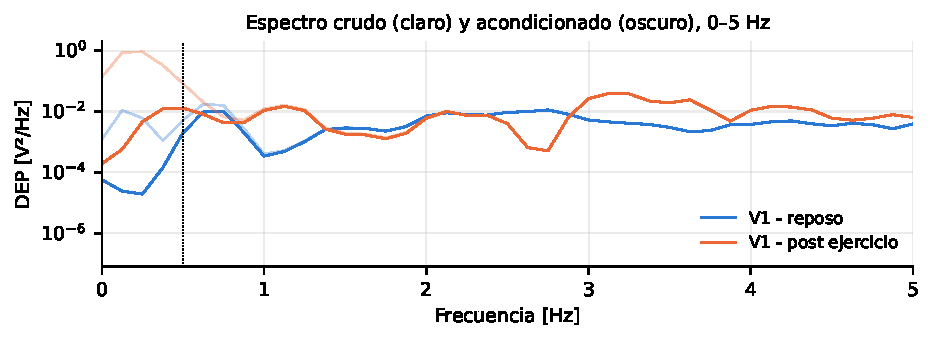
\includegraphics[width=\textwidth]{acond_espectro_antes_despues}
  \caption{Densidad espectral de potencia de 0 a \SI{5}{\hertz} de los registros crudos (trazo claro) y acondicionados (trazo oscuro). La línea punteada marca el corte del pasaaltos.}
  \label{fig:acond_espectro_antes_despues}
\end{figure}

% Plantilla de figura (las figuras las genera guardar_figura() en informe/figuras/)
% \begin{figure}[htbp]
%   \centering
%   \includegraphics[width=\textwidth]{nombre_figura}
%   \caption{...}
%   \label{fig:nombre_figura}
% \end{figure}

\subsection{Detección de latidos}
\label{sec:res-deteccion}
% Responde: ítem 6 (detección)
\pendiente{Etapas de Pan-Tompkins sobre un registro y detecciones en los cuatro registros.}

\subsection{Tacogramas}
\label{sec:res-tacograma}
% Responde: ítems 6a y 6b
\pendiente{Ítem 6a: variación de la frecuencia cardíaca en cada registro.}

\pendiente{Ítem 6b: comparación entre voluntarios.}

\subsection{Análisis espectral}
\label{sec:res-lomb}
% Responde: ítems 7a y 7b
\pendiente{Ítem 7a: diferencias entre reposo y post ejercicio.}

\pendiente{Ítem 7b: comparación entre voluntarios.}
